\documentclass[journal]{IEEEtran}

% --- Packages ---
\usepackage{booktabs}   % For professional looking tables (\toprule, \midrule, \bottomrule)
\usepackage{multirow}   % For spanning cells across multiple rows
\usepackage{pifont}     % For checkmarks and crosses (\ding{51}, \ding{55})
\usepackage{xcolor}     % For coloring checkmarks and crosses
\usepackage{graphicx}   % Graphics insertion
\usepackage{rotating}   % For sidewaysfigure environment
\usepackage{dblfloatfix}% Fixes two-column float queue order and enables [b] on figure*
\usepackage{placeins}   % Keeps floats near their intended sections

% Command definitions for checkmarks and crosses
\newcommand{\cmark}{\ding{51}}
\newcommand{\xmark}{\ding{55}}

% Loosen float placement constraints to avoid figure postponement
\renewcommand{\topfraction}{0.95}
\renewcommand{\bottomfraction}{0.85}
\renewcommand{\textfraction}{0.1}
\renewcommand{\floatpagefraction}{0.8}
\renewcommand{\dbltopfraction}{0.95}
\renewcommand{\dblfloatpagefraction}{0.8}

% Correct bad hyphenation here
\hyphenation{op-tical net-works semi-conduc-tor}

\begin{document}

\title{Episodic Memory for Robots in the Wild: Benchmarking and Evaluation Across Unstructured Environments}

\author{Vedansh~Malhan, \IEEEmembership{Student, Monash University}, William~Ngo, \IEEEmembership{Student, Monash University}
\thanks{Special thanks to Kavi Katuwandeniya and Dana Kuli\'{c} for their support in the research. This work was supported in part by Monash University Engineering Department.}
\thanks{V. Malhan is with the Software Engineering Department, Monash University, Clayton, Melbourne, VIC 3800, Australia (e-mail: vedanshmalhan03@gmail.com).}
\thanks{W. Ngo is with the Department of Electrical and Computer Systems Engineering, Monash University, Clayton, Melbourne, VIC 3800, Australia.}
}

% Paper headers
\markboth{Episodic Memory for Robots in the Wild: Benchmarking and Evaluation Across Unstructured Environments}%
{\MakeLowercase{\textit{et al.}}: Episodic Memory for Robots in the Wild: Benchmarking and Evaluation Across Unstructured Environments}

\maketitle

\begin{abstract}
Vision-Language Models (VLMs) are seeing increased adoption in modern systems such as autonomous vehicles and embodied agents. These systems require a continuous, long-term understanding of past events, known as episodic memory, to maintain task context and prevent operational failures. Despite its critical importance, current benchmarks evaluating episodic memory in VLMs remain limited. Existing datasets typically feature short-duration clips (seconds to minutes) in event-dense environments, characterised by high-frequency occurrences that result in high Signal-to-Noise Ratio (SNR) scenarios. Consequently, there is a significant lack of benchmarks addressing low-SNR, event-sparse environments such as forests, rural roads, and tunnels which demand fine-grained episodic discrimination and long-range temporal retrieval over extended sequences. To address this gap, we propose a benchmarking framework for evaluating episodic memory in modern VLMs in low-SNR environments, utilising extended duration videos ranging from 6 minutes to 1 hour. The framework includes a pipeline for generating natural language query-based question-answer pairs using modern Large Language Models (LLMs) and VLMs, followed by human verification. The benchmark targets three key evaluation categories: sparse-event localisation and temporal ordering. This benchmark is anticipated to provide an evaluation framework capable of exposing the limitations of current multi-modal architectures.
\end{abstract}

% ---------------------------------------------------------
% INTRODUCTION
% ---------------------------------------------------------
\section{Introduction}
\label{sec:introduction}

\IEEEPARstart{R}{ecent} advancements in Vision-Language Models (VLMs) have facilitated their integration into complex, real-world applications, particularly within the autonomous vehicle and robotics industries \cite{kodiak2023}. For these systems to operate reliably, the capacity to retain and retrieve specific past experiences over extended periods is crucial. Originating from cognitive psychology \cite{tulving1972episodic}, episodic memory is defined as the ability to encode, store, and consciously recall specific past events anchored in their precise spatial and temporal contexts. For instance, in autonomous navigation, the inability to recall past road conditions in a GNSS-denied environment poses critical safety risks and compromises localisation capabilities. Similarly, episodic memory in robotics enables long-term continuity, enhanced social interaction, and advanced cognitive planning by allowing agents to store and retrieve specific temporal experiences, rather than relying solely on generalised semantic memory.

Although recent research has benchmarked the temporal and memory capabilities of VLMs, existing datasets, such as Ego4D \cite{ego4d}, predominantly focus on short-duration video clips averaging approximately eight minutes. Furthermore, these datasets are heavily skewed toward event-dense settings characterised by a high Signal-to-Noise Ratio (SNR). In the context of video analysis, SNR refers to the density of meaningful, distinct events (the ``signal'') relative to continuous, repetitive, or uninformative background frames (the ``noise''). Consequently, current benchmarks primarily capture general daily activities in object-rich environments like private homes and offices, where visual stimuli and new events occur almost continuously.

Consequently, a significant gap exists regarding the evaluation of VLMs in low SNR, lengthy-context, and event-sparse environments. Scenarios such as navigating through forests, rural roads, and tunnels present a unique challenge. The absence of distinctive landmarks deprives VLMs of visual anchors; as a result, the context window becomes saturated with highly similar tokens. This homogeneity severely challenges frame-level recall and temporal anchoring. Fine-grained episodic discrimination over extended sequences remains largely untested in current VLM literature.

To address this critical gap, this study is guided by the following research question: \textit{\textbf{Can modern Vision-Language Models accurately recall, distinguish, and reason with episodic memories in an event-sparse environment?}}

The primary objective of this project is to develop a comprehensive and reliable benchmark to assess the episodic memory of VLMs within the aforementioned domains. To achieve this, an automated pipeline is proposed to generate question-answer pairs based on long-form video inputs, which are subsequently validated via human annotation. The benchmark evaluates models across three main categories:
\begin{itemize} 
\item \textbf{Sparse Event Localisation:} Verifying the occurrence of rare, outlier events over extended durations (e.g., identifying a wildlife crossing during a long drive). 
\item \textbf{Temporal Order:} Assessing the model's capacity to recall the chronological sequence of past events. 
\end{itemize}

By exposing vulnerabilities in current architectures, this benchmark aims to push the boundaries of long-term temporal context retention in modern multi-modal models.

\begin{table*}[t]
\centering
\begin{tabular}{lrrrrrcccc}
\toprule
\textbf{Benchmarks} & \textbf{\#Videos} & \textbf{\#Clips} & \textbf{Len.(s)} & \textbf{\#QA Pairs} & \textbf{Anno.} & \textbf{Egocentric} & \textbf{Low-SNR} & \textbf{Long-Horizon} \\
\midrule
% --- Early Benchmarks ---
MSRVTT-QA \cite{msrvtt} & 2,990 & 2,990 & 15.2 & 72,821 & A  & \xmark & \cmark & \xmark \\
TGIF-QA \cite{tgif} & 9,575 & 9,575 & 3.0 & 8,506 & A\&M & \xmark & \cmark & \xmark \\
ActivityNet-QA \cite{activitynetqa} & 800 & 800 & 111.4 & 8,000 & M  & \xmark & \xmark & \xmark \\
\midrule
% --- Recent Benchmarks ---
MVBench \cite{mvbench} & 3,641 & 3,641 & 16.0 & 4,000 & A  & \xmark & \cmark & \xmark \\
EgoSchema \cite{egoschema} & 5,063 & 5,063 & 180.0 & 5,063 & A\&M  & \xmark & \xmark & \xmark \\
\midrule
% --- Video-MME ---
Video-MME-S & 300 & 300 & 80.7 & 900 & \multirow{4}{*}{M}   & \cmark & \cmark & \cmark \\
Video-MME-M & 300 & 300 & 515.9 & 900 & & \cmark & \cmark & \cmark \\
Video-MME-L & 300 & 300 & 2466.7 & 900  & & \cmark & \cmark & \cmark \\
Video-MME \cite{videomme} & 900 & 900 & 1017.9 & 2,700 & & \cmark & \cmark & \cmark \\
\midrule
% --- OUR BENCHMARK ---
\textbf{FYP2026S1-3073} & \textbf{17} & \textbf{17} & \textbf{1800} & \textbf{422} & \textbf{A\&M} & \textbf{\cmark} & \textbf{\cmark} & \textbf{\cmark} \\
\bottomrule
\end{tabular}
\vspace{1ex}
\caption{Comparison of key dataset characteristics across benchmark frameworks: total videos (\textbf{\#Videos}), average length of video input (\textbf{Len.(s)}), total clips (\textbf{\#Clips}), total Question-Answer pairs (\textbf{\#QA Pairs}), and annotation paradigm (\textbf{Anno.}: M for manual, A for automated).}
\label{tab:benchmark_comparison}
\end{table*}

% ---------------------------------------------------------
% RELATED WORK
% ---------------------------------------------------------
\section{Related Work}
\IEEEPARstart{T}{he} capabilities of Vision Language Models (VLMs) and their temporal reasoning abilities have seen massive growth in recent years through the development of transformers. 

Early video question answering benchmarks such as \textbf{TGIF} \cite{tgif}, \textbf{Movie-QA} \cite{movieqa}, and \textbf{ActivityNet-QA} \cite{activitynetqa} laid the groundwork for temporal reasoning in VLM architectures. Subsequent efforts expanded into instructional and narrated content, with datasets like \textbf{HowTo100M} \cite{howto100m} and \textbf{CrossTask} \cite{crosstask} evaluating the alignment of spoken language with visual steps. However, these datasets primarily consist of brief clips, typically ranging from a few seconds to five minutes, which are insufficient for testing long-term memory retention.

More recently, the focus in benchmarks has shifted towards comprehensive, long-context video evaluations. Benchmarks such as \textbf{Video-MME} \cite{videomme}, \textbf{LongVideoBench} \cite{longvideobench}, and \textbf{EgoSchema} \cite{egoschema} provide extensive multi-modal evaluations across longer durations. While these benchmarks test temporal contexts, they are fundamentally built upon high-SNR environments (e.g., movies, vlogs, and television shows) where distinct visual and audio cues occur with high frequency. Furthermore, these datasets are primarily sourced from third-person media, limiting their applicability to autonomous vehicles and robotics, which inherently rely on egocentric viewpoints to perform real-world tasks.

In the context of egocentric vision and embodied AI, the current frontier includes benchmarks like \textbf{Ego4D} \cite{ego4d}, which evaluates egocentric video understanding via body-mounted cameras. In simulated environments, benchmarks such as \textbf{Embodied Question Answering} \cite{embodiedqa}, \textbf{House3D} \cite{house3d}, and \textbf{Enter the Mind Palace} \cite{mindpalace} assess spatial and episodic memory for embodied agents. While highly influential, these datasets generally remain focused on human activities that are high SNR and bounded by synthetic simulations. Similarly, in the autonomous driving domain, \textbf{NuScenes QA} \cite{nuscenesqa} and \textbf{The Blind Spot of Adaptation} \cite{blindspot} benchmark episodic memory in autonomous vehicles, but strictly focus on dense, high-SNR urban traffic rather than feature-sparse environments.

Despite these advancements across adjacent domains, a critical gap remains. Prior work covers complementary facets of this problem: Video-MME, LongVideoBench, and EgoSchema evaluate long-context video QA; Ego4D provides an egocentric viewpoint; and NuScenes-QA addresses autonomous driving scenes. This study targets their intersection: extended, forward-facing vehicle trajectories with sparse salient events, evaluated using AI-annotated and human-reviewed questions covering rare-event identification and chronological event sequencing.

% ---------------------------------------------------------
% METHODOLOGY
% ---------------------------------------------------------
\section{Methodology}
\label{app:methodology}

We present a benchmark for assessing the episodic memory of Vision-Language Models (VLMs) in long, egocentric dashcam recordings. Each recording is a forward-facing vehicle camera sequence filmed at 10~FPS, ranging from 15 minutes to an hour in duration, captured in low event-density environments such as forests and rural roads. These environments exhibit few stable visual landmarks; consequently, answering queries across such trajectories requires recalling context across long temporal horizons rather than relying on isolated frame observations. The benchmark targets two primary categories:
\begin{enumerate}
    \item \textbf{Sparse event localisation}, which evaluates whether a model can verify rare, outlier events without hallucinating non-existent occurrences.
    \item \textbf{Temporal order}, which tests whether a model recalls the exact chronological sequence of events rather than inferring order from environmental priors.
\end{enumerate}

\subsection{Data Source and Preparation}

\begin{figure}[t]
    \centering
    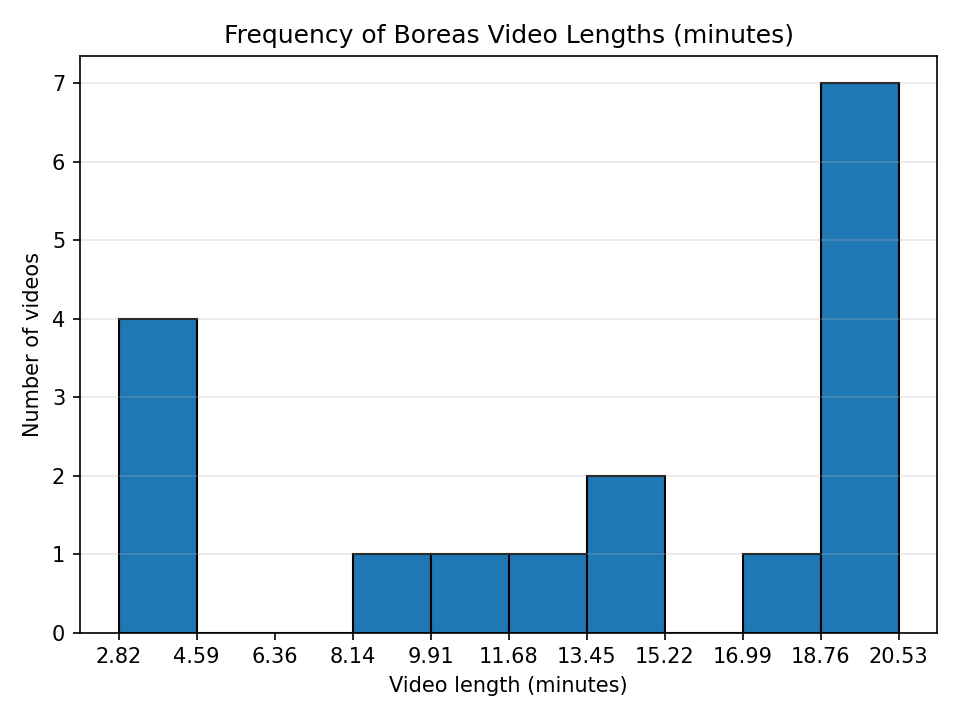
\includegraphics[width=\columnwidth]{boreas_video_length_frequency.png}
    \caption{Distribution of video sequence durations across the extracted Boreas dataset segments.}
    \label{fig:boreas_length_dist}
\end{figure}

Source frames are collected from the Boreas dataset \cite{burnett2023boreas} (covering tunnel and rural sequences) and the CSIRO forest dataset (K-01) \cite{csiro_k01_forest}. As shown in Fig.~\ref{fig:boreas_length_dist}, the Boreas trajectories exhibit a wide temporal spread ranging from short segments under 5 minutes to long sequences exceeding 20 minutes, with the majority clustering around extended durations. Each frame is an individual image whose filename encodes its capture timestamp in epoch microseconds (e.g., \texttt{1733343593917869.png}). Elapsed time is computed directly from these timestamps rather than inferred from video metadata or playback speed.

Due to the substantial length of the source videos (averaging $\sim$45 minutes), fully manual annotation presented significant scalability bottlenecks, particularly regarding the identification of sparse events and the tracking of multi-event temporal dependencies. Consequently, a semi-automated annotation framework was adopted: GPT-6-Luna was deployed to generate initial candidate events and segment boundaries, which were subsequently audited and refined through expert human review to prevent hallucinations and establish reliable ground-truth labels.

\subsection{Temporal Sliding-Window Partitioning}

Direct ingestion of a complete 45-minute video sequence of 4K frames in a single inference pass is computationally intractable, as the resulting token volume exceeds the context window limits of contemporary Vision-Language Models (VLMs). To operate strictly within model context boundaries and manage token expenditure, a temporal sliding-window partitioning mechanism was deployed.

Under this framework, the continuous video stream is partitioned into discrete temporal segments parameterized by three primary variables:
\begin{itemize}
    \item \textbf{Window capacity ($W$):} The number of frames ingested per processing segment.
    \item \textbf{Stride ($S$):} The temporal displacement between consecutive evaluation windows.
    \item \textbf{Subsampling interval ($\delta$):} A frame-skip parameter applied across temporal sequences.
\end{itemize}

Because the underlying video stream is recorded at a native capture rate of 10~Hz, inter-frame visual redundancy is high; variations across short intervals ($\le 4$~frames, or $\sim 0.4$~s) rarely exhibit salient state transitions. Introducing uniform temporal skipping therefore provides an optimal trade-off between token conservation and temporal resolution without compromising semantic event capture.

Furthermore, because downstream benchmark evaluation is restricted to multiple-choice question (MCQ) formulations, evaluation items are grounded strictly within the temporal boundaries of the extracted and verified segments. This guarantees that model queries are never issued over unobserved intervals, eliminating ungrounded negative evaluations and maintaining the integrity of the ground-truth benchmark.

\subsection{Ground-Truth Construction}

Ground truth is constructed across four sequential stages (summarised in Fig.~\ref{fig:sparse_temporal_pipeline}), where each stage is decoupled and validated by an expert reviewer prior to proceeding.

\subsubsection{Candidate Extraction}
A VLM receives the frames of each partitioned section alongside a task-specific prompt and returns structured JSON \cite{burnett2023boreas}. In the sparse task, the prompt instructs the model to detect noteworthy, anomalous events while ignoring routine driving sequences. In the temporal task, the prompt extracts a section summary and a chronological sequence of timestamped events. Each extracted event is mapped to \texttt{start\_seconds} and \texttt{end\_seconds} derived from the manifest file of the section.

\subsubsection{Deterministic Ordering and LLM-Assisted Merging}
Candidate detections are sorted chronologically via frame timestamps. The sorted manifest is written to \texttt{all\_results.json} and batched into an LLM using sliding review windows (\texttt{review\_window} for sparse, \texttt{merge\_window} for temporal tasks). For the sparse task, the LLM merges duplicate detections spanning consecutive window boundaries and flags spurious false positives with accompanying justifications. For the temporal task, the LLM links continuous observations while preserving strict sequence integrity. Timestamps are re-anchored to the verified records, yielding consolidated outputs stored in \texttt{events.json} and \texttt{timeline.json}.

\subsubsection{Human Verification}
A human reviewer inspects each candidate entry against the source video frames, pruning erroneous detections and refining temporal boundaries. Only verified entries are admitted into question generation. For the temporal task, a synthesized prose storyline is compiled to accelerate manual audit.

\subsubsection{Question Generation}
The LLM synthesizes evaluation questions exclusively from the verified candidate pool. Each item includes its question typology, target event IDs, supporting frame identifiers, answer options, and the verified index of the ground truth.

\subsection{Question Design}

\textbf{Sparse event localisation.} Three question typologies are generated:
\begin{itemize}
    \item \emph{Deceptive:} Queries whether an invented, plausible event occurred (correct answer is always negative). Invented events are sampled without replacement across questions to prevent inter-query inference leakage.
    \item \emph{Existence:} Inquires whether a confirmed, verified event occurred during the sequence (correct answer is affirmative).
    \item \emph{Noteworthy:} Presents four candidate events, consisting of exactly one verified occurrence and three plausible distractors.
\end{itemize}
Invented events are tracked within an auxiliary \texttt{false\_events} schema alongside their assigned \texttt{question\_id} and generation rationale to facilitate negative-instance verification.

\textbf{Temporal order.} Three question typologies evaluate sequential understanding:
\begin{itemize}
    \item \emph{Pairwise order:} Evaluates relative temporal precedence between two discrete events.
    \item \emph{Sequence order:} Requires arranging three to five distinct events in valid chronological succession.
    \item \emph{Before/after:} Queries which event immediately preceded or succeeded a reference milestone.
\end{itemize}

\begin{table}[!t]
\centering
\begingroup
\scriptsize
\setlength{\tabcolsep}{2pt}
\resizebox{\columnwidth}{!}{%
\begin{tabular}{lrrrrr}
\toprule
\textbf{Group} & \textbf{\#Videos} & \textbf{Mean (min)} & \textbf{Sparse QA} & \textbf{Temporal QA} & \textbf{Total QA} \\
\midrule
Short & 5 & 4.74 & 60 & 65 & 125 \\
Medium & 4 & 13.03 & 51 & 50 & 101 \\
Long & 8 & 19.16 & 113 & 105 & 218 \\
\midrule
All & 17 & 13.47 & 224 & 220 & 444 \\
\bottomrule
\end{tabular}
}% resizebox
\endgroup
\caption{Duration-stratified composition of the 17 video sequences. Short: $t \leq 10$ min; medium: $10 < t \leq 15$ min; long: $t > 15$ min. Durations are measured from camera-frame timestamps.}
\label{tab:duration_composition}
\end{table}
\FloatBarrier

\subsection{Selection of Evaluation Categories}
The overall design of the benchmark reflects the operational demands of autonomous agents in low-SNR environments:
\begin{itemize}
    \item \textbf{Sparse Event Localisation:} Under extended, featureless driving conditions, detecting rare anomalies is critical for safety and state estimation.
    \item \textbf{Temporal Ordering:} Long-horizon navigation requires maintaining an accurate internal timeline of sequential milestones rather than relying on frequency heuristics.
\end{itemize}

% ---------------------------------------------------------
% RESULTS
% ---------------------------------------------------------
\section{Discussion}

In this section, we'll evaluate the result from various different VLM models to assess them on how they go against our Episodic Memory benchmark.

We conducted the test on various VLM models from the top well known companies. Some closed source models include 

\appendices

\ifCLASSOPTIONcaptionsoff
  \newpage
\fi

\bibliographystyle{IEEEtran}
\bibliography{bibtex/bib/References}

\end{document}
